% !TeX root = ../full_report.tex

\chapter{State of the art}
\section{SIFT and bag-of-words}
Until recently, the state of the art in image retrieval and matching
was based on the idea of
bag-of-words~\cite{philbin_object_2007}~\cite{mikulik_learning_2013}.
The idea behind the approach is to represent an image as a histogram,
or collection of frequencies, of visual words. The visual words should
be small, representative patches of the images in the dataset.
Usually, these visual words are obtained in multiple steps. First,
local features are extracted and encoded. The most common feature used
is SIFT~\cite{lowe_distinctive_2004}, a 128-dimensional vector representing
scale-invariant features. Then, the features are extracted for all
images and clustered into clusters of similar features.
The representative for each cluster is the center of the cluster,
i.e. the mean of all features falling into that cluster.
Each image can then be represented as a histogram of the occurrences
of these representative features.
This histogram forms the image descriptor, which has as many dimensions
as there are representative features and clusters.

Finally, for image classification, a classifier can be learned from the
descriptors of all images in the dataset. On the other hand, for image
retrieval or matching, the descriptors can be directly matched against
each other, based on some similarity measure.
In both cases, it can be useful to project the descriptors into a Hilbert
space using a different similarity measure than euclidean distance
in the original descriptor space.
For classification, this is done by employing an SVM classifier with a
non-linear kernel~\cite{shawe-taylor_kernel_2004}.
Among the most popular kernels are the
radial basis function~\cite{scholkopf_comparing_1997}
and the chi-squared function~\cite{vedaldi_efficient_2012}.

Until recently, this approach has obtained state of the art results for
image retrieval tasks~\cite{mikulik_learning_2013}.

\section{Deep learning with CNNs}
Starting with the results of AlexNet for image classification in the 2012
ImageNet challenge~\cite{krizhevsky_imagenet_2012}
~\cite{russakovsky_imagenet_2015},
image classification tasks have been dominated by CNNs, learned using
large amounts of data.

A general trend in image related tasks is to move to an end-to-end
approach, where the final objective is directly optimized using gradient
descent and the gradient is back-propagated to all previous parts of the
system. In contrast, the bag-of-words model requires a choice of
features (SIFT, ORB (TODO mention ORB before), \dots),
a choice of the method for clustering features (k-means),
a choice of the classifier (AdaBoost~\cite{freund_desicion-theoretic_1995},
SVM, \dots), as well as a choice of the kernel if an SVM classifier is used.

Using a CNN, features are extracted at a low abstraction level by the
first convolutional layers, then higher level features are formed
by combining low level features from the previous layers. Finally,
high-level features are combined into a classifier by linear layers.
The advantage of this approach is that the features are learned at all
abstraction levels. Furthermore, the modularity of the approach allows
us to easily transfer the lower level features learned from a large dataset
to a smaller dataset, where there may not be enough data to efficiently
learn lower level features.

The following sections describe the high-level architecture of the
most widely used CNNs in classification and image retrieval.
\subsection{AlexNet}
AlexNet~\cite{krizhevsky_imagenet_2012} contains five convolutional
layers and three linear layers. The first convolutional layer
has a large kernel and stride to quickly increase the receptive field
of the consequent filters. The first two convolutional layers are followed
by a pooling layer to further increase the receptive field.

Finally, an important improvement for AlexNet to avoid over-fit is
the addition of dropout layers~\cite{hinton_improving_2012} before the
two first linear layers.

Apart from that, AlexNet is a simple adaptation of LeNet by
LeCun et al~\cite{lecun_gradient-based_1998} for the ImageNet challenge.

\subsection{VGG}
The VGG architecture, introduced by Simonyan et al~\cite{simonyan_very_2014}
is the first to use exclusively $3\times3$ convolutional kernels.
This means that the receptive field of the
first filters is much smaller, and thus many more layers are needed,
as well as more pooling layers. The most popular VGG architectures
are VGG-16 and VGG-19, having 16 and 19 layers in total respectively.

Using smaller kernels in convolutions and consequently more layers
allows to reduce the number of trainable parameters used by the
network, while increasing the number of non-linear layers.
This was shown to allow better generalization properties, and thus less
over-fit~\cite{simonyan_very_2014}.

\subsection{ResNet, Inception, DenseNet}
The idea of increasing the number of layers is further developed
by the ResNet, DenseNet and Inception architectures. However,
naively increasing the number of layers leads to the problem of
vanishing gradient~\cite{hinton_fast_2006}.

All of these networks overcome the vanishing gradient problem by
introducing skip connections, where the output of a previous layer
is added to the output of a layer, skipping some number of layers in
between.

The ResNet architecture by He et al~\cite{he_deep_2015} always uses blocks
of 3 layers along with a skip of those 3 layers. The smaller types of
ResNet use blocks of 2 layers.

The Inception architecture by Szegedy et al~\cite{szegedy_inception-v4_2016}
uses a combination of skip connections of different length and different
types.

Finally, DenseNet by Huang et al~\cite{huang_densely_2016} takes the
skip connection idea one step further:
the input of each layer is dependent on the output of all $n$ previous layers
to some extent.

Finally, all of the very deep architectures use batch norm layers to further
reduce over-fit: a batch norm layer simply normalizes the features over each
batch, and then applies a learnable scaling and shifting.

\section{Image retrieval using CNNs}
For image retrieval, the current state of the art is set by
Gordo et al~\cite{gordo_deep_2016}. It is based on an
end-to-end approach. The goal is to learn a global descriptor for images
that is well suited for comparing images.

\begin{figure}
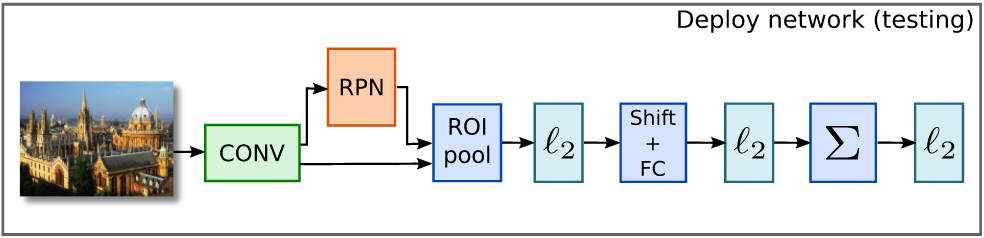
\includegraphics[width=\textwidth]{img/gordo_deepimageretrievaldeploy.png}
\caption{Architecture of a CNN network for image retrieval
\label{fig:gordo_deploy}}
\end{figure}
Figure~\ref{fig:gordo_deploy} shows the detailed architecture used.
It first extracts the convolutional features of a pre-trained
CNN. Then, a Region Proposal Network (RPN)~\cite{ren_faster_2015} is
used to extract the regions of interest. For each region of interest,
a shifting and linear layer are used to reduce the dimensionality of
the descriptor. The final descriptor is simply a normalized sum of the
region-wise descriptors. This network can be learned end-to-end and
the obtained descriptor achieves state of the art results, which can
be even further improved by using query expansion and database side
feature augmentation (TODO either remove or mention before).

Gordo et al~\cite{gordo_deep_2016} found that using very deep networks
outperforms the shallower networks. The state of the art results are
thus set by a very deep ResNet architecture.

\subsection{Siamese networks and triplet loss}
\begin{figure}
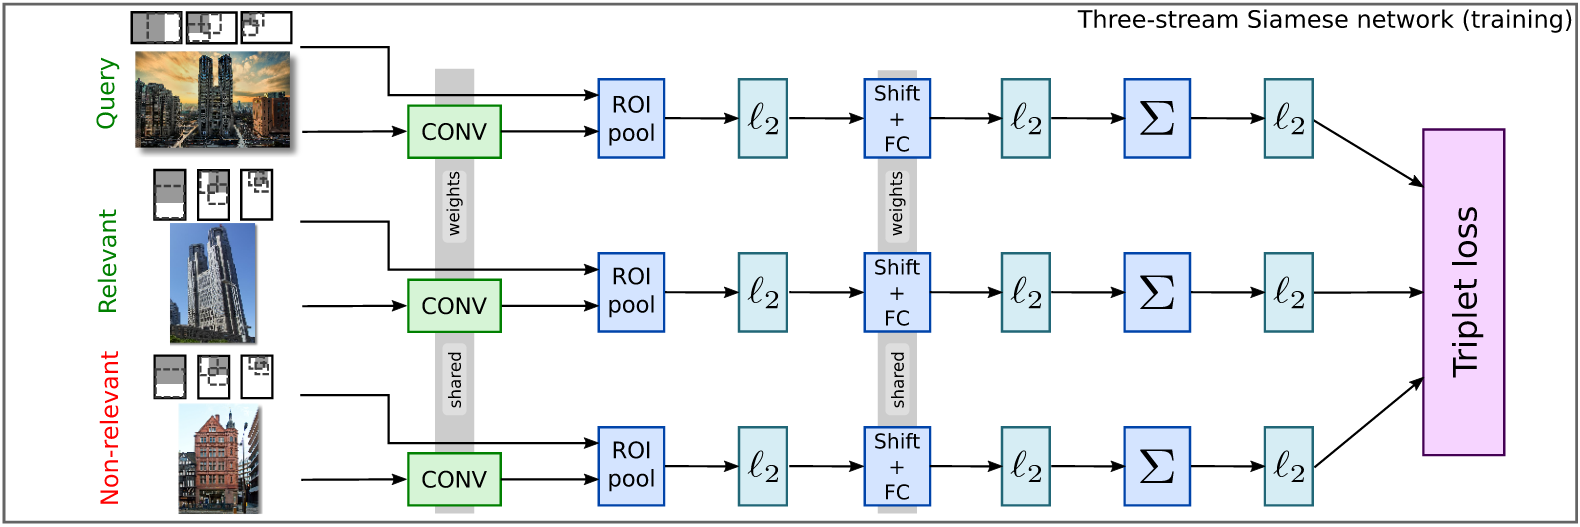
\includegraphics[width=\textwidth]{img/gordo_deepimageretrievalarc.png}
\caption{Siamese architecture of a CNN for image retrieval used in training
\label{fig:gordo_train}}
\end{figure}

Figure~\ref{fig:gordo_train} shows the architecture used to train the CNN
that produces a descriptor for images, as can be seen in
Figure~\ref{fig:gordo_deploy}.

The major difference is that during training, a Siamese architecture is
used: the CNN is evaluated with multiple images, using the same weights
for each. Then, a combined loss is obtained from the descriptors.
Finally, the loss is back-propagated once through all streams of the network,
since shared weights are used for all images.

In the case of this particular architecture, three images are evaluated
and a triplet loss is used. This triplet loss has previously been used
in face recognition tasks by Schroff et al~\cite{schroff_facenet:_2015}.
The triplet loss was first introduced by
Weinberger et al~\cite{weinberger_distance_2006} as a way of learning
the best suited distance metric in a k-nearest neighbor classification
problem.
